\documentclass[11pt,a4paper,twoside]{article}
\usepackage[utf8]{inputenc}
\usepackage[T1]{fontenc}

\usepackage{mathptmx}
\usepackage{datetime}
\usepackage[spanish, es-nolists]{babel}
\usepackage{amsmath}
\usepackage{amsthm}
\usepackage{amsfonts}
\usepackage{amssymb}
\usepackage{titlesec}
\usepackage{graphicx}
\usepackage{mathtools}

\decimalpoint

\usepackage{array}
\usepackage{float}
\usepackage[a4paper]{geometry}
\geometry{top=2.5cm, bottom=2cm, left=2.54cm, right=2.54cm}
\usepackage{fancyhdr}
\pagestyle{fancy}
\fancyhf{}  % Limpiar los encabezados y pies de página predeterminados
% Encabezados para páginas impares
\fancyhead[LE,RO]{\thepage} % En la izquierda de la página impar
\fancyhead[RE]{\textsc{Garbayo, I.}} % En la derecha de la página impar
% Encabezados para páginas pares
\fancyhead[LO]{\textit{Generación y optimización de código}}  % En la izquierda de la página par
\fancyfoot{}

\usepackage{color}
\usepackage{cancel}
\usepackage{ulem}
\usepackage{tcolorbox}
\usepackage{multirow}
\usepackage{tikz}
\usetikzlibrary{babel, arrows.meta, arrows, datavisualization, patterns}
\usepackage{multicol}
\usepackage{stackrel}
\usepackage{pdfpages}
\renewcommand{\labelitemi}{\textbullet}

\theoremstyle{definition}
\newtheorem{ejemplo}{\textbf{Exemplo}}
\newtheorem{ejer}{\textcolor{red}{\textbf{Exercicio}}}
\newtheorem{defi}{\textbf{Definición}}
\newtheorem{theorem}{\textbf{Teorema}}
\newtheorem{lema}{\textbf{Lema}}
\newtheorem{corol}{\textbf{Corolario}}
\newtheorem{prop}{\textbf{Proposición}}
\newtheorem{nota}{\textbf{\textit{Nota}}}

\renewcommand\qedsymbol{$\blacksquare$}

\usepackage{hyperref}
\hypersetup{
	colorlinks,
	citecolor=black,
	filecolor=black,
	linkcolor=black,
	urlcolor=black
}

\usepackage{enumitem}


\newcommand{\imagen}[1]{
	\begin{figure} [H] \centering
		\includegraphics[width=\textwidth]{#1}
	\end{figure}
}

\title{%
	\LARGE \textbf{Compiladores e Intérpretes} \\ \vspace*{1cm} \textbf{Práctica 2: Generación y optimización de código}
	\\ \Large \textbf{\textsc{Optativa}. \textit{Peeling} de lazos}}
\author{\textsc{Ignacio Garbayo Fernández}}
\date{Universidade de Santiago de Compostela}

\setlength{\parskip}{5pt}

\usepackage{setspace}

%\onehalfspacing % Configura el interlineado a 1.5

\setlength{\parindent}{0.7cm}

\usepackage[hang, small,labelfont=bf,up,textfont=up]{caption}
\usepackage{hanging}
\usepackage{sectsty}

\sectionfont{\fontsize{14}{15}\selectfont}
\subsectionfont{\fontsize{12}{15}\selectfont}
\subsubsectionfont{\fontsize{12}{15}\selectfont}

\usepackage{titlesec}
\titleformat{\subsection}[block]{\normalfont\large\itshape}{\thesubsection}{1em}{}
\titlespacing*{\section}
{0pt}{\baselineskip}{0pt}
\titlespacing*{\subsection}
{0pt}{\baselineskip}{0pt}
\titlespacing*{\subsubsection}
{0pt}{\baselineskip}{0pt}

\usepackage[cache=false]{minted}
\definecolor{bg}{rgb}{.95, .95, .95}

\usepackage[backend=biber, style=ieee, sorting=nty]{biblatex}
\bibliography{references}


\begin{document}
	
	% PORTADA
	\maketitle
	\thispagestyle{empty}
	
	\vspace*{1cm}
	
	% ÍNDICE
	\renewcommand{\contentsname}{Índice} % Cambia el título
	\tableofcontents


	\newpage


	\section{Introducción}
	
	El \textit{peeling} de lazos es una técnica de transformación utilizada en la optimización de código generada por compiladores. Consiste en extraer una o más iteraciones iniciales (o finales) de un bucle y tratarlas por separado, fuera del cuerpo principal del mismo. Esta transformación puede parecer trivial a primera vista, pero resulta esencial en numerosos contextos donde la regularidad del bucle o la presencia de dependencias condicionan el rendimiento del código ejecutable.
	
	Entre sus principales objetivos se encuentran la eliminación de dependencias que impiden optimizaciones posteriores (como la vectorización), la alineación de accesos a memoria, y la especialización de ciertas iteraciones con comportamiento no homogéneo. Desde el punto de vista del rendimiento, el \textit{peeling} puede introducir un pequeño aumento en el tamaño del código debido a la duplicación parcial de instrucciones, pero a cambio permite a los compiladores generar versiones más eficientes del bucle principal.
	
	El objetivo principal del estudio es implementar dicha optimización sobre el código proporcionado, evaluar su impacto en el rendimiento y analizar su escalabilidad con respecto al tamaño del problema y al número de repeticiones (\texttt{ITER}). Para obtener medidas fiables, se realizan múltiples ejecuciones de cada versión del código (con y sin optimización), compiladas con el nivel de optimización \texttt{-O0} para evitar interferencias de otras transformaciones automáticas del compilador. Asimismo, se analiza el código ensamblador generado con el fin de confirmar que la sustitución ha tenido efecto y para entender mejor las diferencias observadas en los tiempos de ejecución.
	
	La práctica se completa con una interpretación de los resultados experimentales y un estudio de cómo influyen factores como la memoria caché y el número de repeticiones sobre la estabilidad y precisión de las medidas de tiempo, aportando una visión más completa sobre los beneficios reales de aplicar esta optimización.
	

	\section{Descripción de la técnica}

	Los bucles en los programas son la fuente de muchas optimizaciones que conducen a mejoras en el rendimiento, particularmente en arquitecturas modernas de alto rendimiento, así como en sistemas vectoriales y multihilo. Entre las técnicas de optimización, el \textit{peeling} de lazos es una técnica importante que puede utilizarse para paralelizar los cálculos. Esta técnica se basa en mover los cálculos de las iteraciones tempranas fuera del cuerpo del bucle, de manera que las iteraciones restantes puedan ejecutarse en paralelo. Un tema clave en la aplicación del \textit{peeling} de lazos es la cantidad de iteraciones que deben extraerse del cuerpo del bucle. Las técnicas actuales utilizan heurísticas o métodos \textit{ad hoc} para «pelar» un número fijo de iteraciones o un número especulado de iteraciones, según se expone en el \cite{art}.
	
	Si solo se separa una iteración, que es un caso común, el código para esa iteración puede incluirse dentro de una instrucción condicional. Si se efectúa el cambio sobre varias iteraciones, puede ser posible utilizar un bucle separado para esas iteraciones. Los principales objetivos de esta técnica son eliminar las dependencias que las iteraciones tempranas crean sobre las iteraciones restantes, lo que permite la paralelización, y ajustar el control de las iteraciones de bucles adyacentes para posibilitar su fusión.
	
	En la Figura \ref{fig:art1} aparecen tres ejemplos de bucles sobre los que se puede aplicar \textit{peeling} para conseguir paralelismo o vectorizaciones, salvando así las dependencias entre los valores.
	
	\begin{figure} [H] \centering
		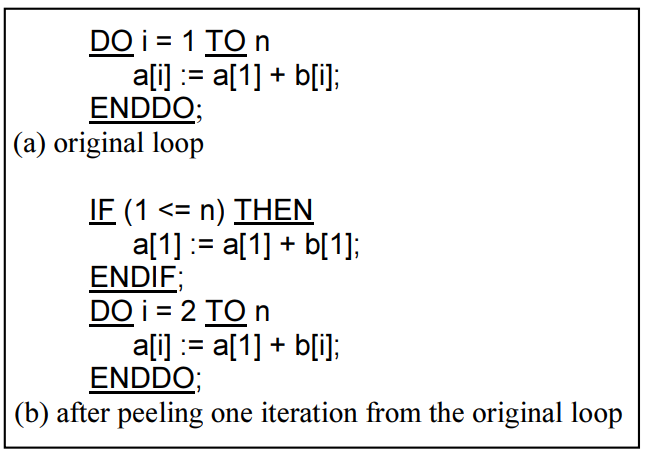
\includegraphics[width=.31\textwidth]{art1.png}
		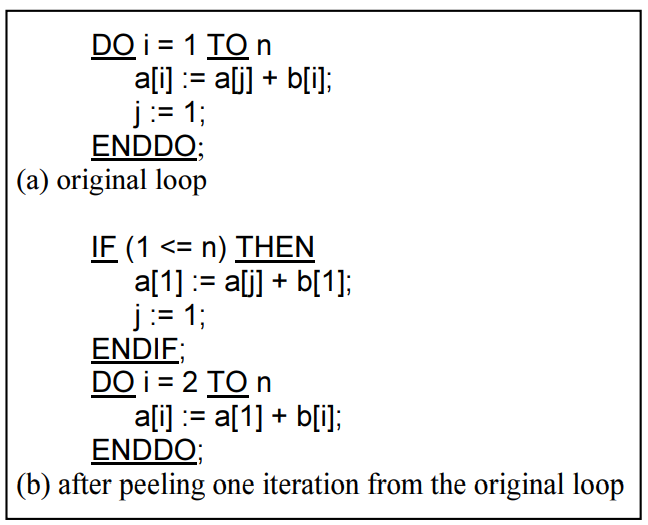
\includegraphics[width=.31\textwidth]{art2.png}
		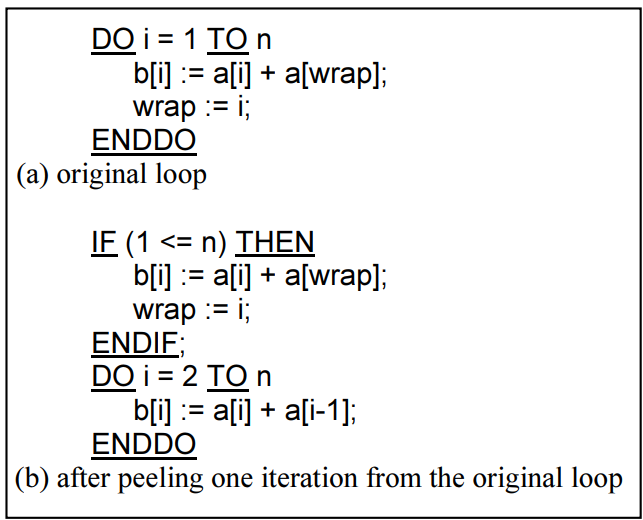
\includegraphics[width=.31\textwidth]{art3.png}
		\caption{Tres ejemplos donde aplicar \textit{peeling} permite optimizar el código.}
		\label{fig:art1}
	\end{figure}
	
	Para la práctica, se propone estudiar en primera instancia el rendimiento de la siguiente porción de código.
	
	\begin{minted}[linenos, fontsize=\small, bgcolor=bg]{c}
for(k=0; k<ITER; k++) {
	for(i=0; i<N; i++) {
		if(i == N/2) { x[i] = 0; }
		else if(i == N-1) { x[i] = N-1; }
		else { x[i] = x[i] + y[i]; }
	}
}
	\end{minted}

	En segundo lugar, se aplicará \textit{peeling} en las iteraciones media y final, según el siguiente bloque, que permite eliminar las sentencias condicionales del algoritmo.
	
	\begin{minted}[linenos, fontsize=\small, bgcolor=bg]{c}
for(k = 0; k<ITER; k++) {
	for(i = 0; i<N/2; i++) { x[i] = x[i] + y[i]; }
	x[N/2]=0;
	for(i = N/2 + 1; i<N - 1; i++) { x[i] = x[i] + y[i]; }
	x[N - 1] = N - 1;
}
	\end{minted}
	
	Para ambas versiones, se explica a continuación la motivación de los 2 bucles anidados exteriores.
	
	\subsection{Configuración del experimento}
	
	El objetivo del experimento es analizar el comportamiento de la versión original frente a la versión con \textit{peeling} de 2 iteraciones. Para esto, se crea un \textit{array} de valores de \texttt{N} con un número de datos suficiente (39 valores diferentes) y evitando potencias enteras de 2. El \textit{array} se muestra en (\ref{eq:n}).
	
	\begin{equation}\label{eq:n}
		\begin{aligned}
			\texttt{N} = \left(
			\begin{matrix}
				3000,      & 4500,      & 7000,      & 9500,      & 12000,		\\
				17000,     & 25000,     & 34000,     & 40000,     & 56000,		\\
				78000,     & 95000,     & 110000,    & 160000,    & 250000,		\\
				320000,    & 390000,    & 570000,    & 820000,    & 1000000,	\\
				1190000,   & 1500000,   & 1750000,   & 1990000,   & 2550000,	\\ 
				3190000,   & 4200000,   & 5100000,   & 5900000,   & 7800000,	\\
				9500000,   & 11800000,  & 15900000,  & 23900000,  & 53000000,	\\
				95000000,  & 199000000, & 383000000, & 959000000. &	\\
			\end{matrix}
			\right).
		\end{aligned}
	\end{equation}

	Además, resulta importante incluir un bucle externo de número fijo de iteraciones (\texttt{ITER}) cuando se estudia el rendimiento de un algoritmo en función del tamaño del problema, especialmente si este es variable, para garantizar condiciones comparables entre ejecuciones con distintos valores de \texttt{N}. Para valores pequeños de \texttt{N}, la ejecución del algoritmo es demasiado rápida. Esto puede provocar medidas ruidosas y poco precisas por debajo del umbral de resolución del reloj del sistema, aparte de un dominio del \textit{overhead} de la llamada al sistema o del propio cronómetro (si este no valiese 0).
	
	Sin embargo, para valores grandes de tamaño del problema, el algoritmo tarda más, pero con mucha menor variabilidad relativa. Esto genera datos incomparables y gráficas sesgadas. Se introduce así un bucle externo de \texttt{ITER} repeticiones, donde \texttt{ITER} se elige dinámicamente para que el producto $\texttt{ITER} \cdot \texttt{N}$ sea constante (o aproximadamente constante). Fijando que cada repetición del experimento deba tardar, al menos, una decena de segundos, generamos el vector de \texttt{ITER} según (\ref{eq:ITER}), que garantiza esta condición.
	
	\begin{equation} \label{eq:ITER}
		\forall i \in \lbrace 1, \dots, 39 \rbrace, \:\: \texttt{ITER}_i = \left\lfloor \dfrac{7.000.000.000}{\texttt{N}_i} \right\rfloor.
	\end{equation}

	Para el vector (\ref{eq:n}), los valores corrrespondientes se reflejan en (\ref{eq:ejITER}).
	
	\begin{equation} \label{eq:ejITER}
		\begin{aligned}
			\texttt{ITER} = \left(
			\begin{matrix}
				2133333, & 1422222, & 914285, & 673684, & 533333, \\
				376470, & 256000, & 188235, & 160000, & 114285, \\
				82051, & 67368, & 58181, & 40000, & 25600, \\
				20000, & 16410, & 11228, & 7804, & 6400, \\
				5378, & 4266, & 3657, & 3216, & 2509, \\
				2006, & 1523, & 1254, & 1084, & 820, \\
				673, & 542, & 402, & 267, & 120, \\
				67, & 32, & 16, & 6. &  \\
			\end{matrix}
			\right).
		\end{aligned}
	\end{equation}

	Para cada valor de \texttt{N}, es fundamental ejecutar el algoritmo un número suficiente de veces, denotado por \texttt{REPS}, con el fin de obtener medidas de rendimiento representativas y estables. La variabilidad inherente al sistema ---debido a factores como la planificación del sistema operativo, el estado de la caché, o procesos en segundo plano--- puede provocar fluctuaciones significativas en los tiempos de ejecución individuales. Al repetir las mediciones y calcular posteriormente estadísticas como la \textbf{media}, el \textbf{máximo} y el \textbf{mínimo}, se obtiene una caracterización más completa del comportamiento del algoritmo. Estas métricas permiten representar en las gráficas no solo la tendencia central, sino también la dispersión y los extremos del rendimiento, ofreciendo una visión más realista y robusta para comparar implementaciones o analizar cuellos de botella. Para este particular, \texttt{REPS} se fija a 15.
		
	
	\section{Beneficios y desventajas esperados}
	
	La técnica de \textit{loop peeling}, aplicada en este caso a los bucles con condiciones específicas como $i = N/2$ e $i = N - 1$, tiene como principal ventaja la eliminación de ramas condicionales dentro del bucle. Al tratar estos casos especiales de manera separada, se evita la penalización por salto en el flujo de control durante la ejecución. Esto permite que el procesador pueda predecir mejor las instrucciones y optimizar el uso del \textit{pipeline}, lo cual, a su vez, mejora la eficiencia en términos de ciclos de CPU. Además, al separar los casos especiales del bucle general, se facilita la aplicación de técnicas de optimización como la vectorización, que pueden ser beneficiosas en operaciones de procesamiento de datos a gran escala.
	
	Sin embargo, esta técnica tiene también sus desventajas. La principal es la duplicación de código, ya que se repite la lógica de actualización de los elementos del array $x$ en cada uno de los casos ($i = N/2$ e $i = N - 1$). Esto no solo aumenta el tamaño del código, sino que puede complicar el mantenimiento y la comprensión del código a largo plazo, sobre todo si se modifica la lógica del bucle en el futuro. Además, el rendimiento de esta técnica depende de la naturaleza de los bucles y la cantidad de iteraciones especiales. Si el número de iteraciones que caen en los casos especiales es pequeño en comparación con el total de iteraciones, los beneficios de \textit{loop peeling} pueden no ser significativos. En algunos casos, el costo de las instrucciones adicionales y la duplicación del código pueden contrarrestar los beneficios.
	
	A pesar de estas desventajas, en muchos contextos, como en algoritmos numéricos o de procesamiento intensivo de datos, las ganancias de rendimiento obtenidas mediante la optimización del flujo de control pueden superar los inconvenientes. Además, cuando el tamaño del bucle es grande y las iteraciones especiales son más frecuentes, \textit{loop peeling} puede resultar en mejoras de rendimiento sustanciales, especialmente en arquitecturas de procesador modernas que optimizan el uso de caché y el paralelismo.
	
	
	\section{Programación y código en ensamblador}
	
	\subsection{Arquitectura de compilación y ejecución}
	
	La compilación con la opción \texttt{-S} de GCC produce códigos fuente del ensamblador de la máquina mediante los que podemos analizar la traducción de las 2 estrategias. Se han ejecutado los códigos en una máquina ASUS Zenbook UX425EA 1.0, equipada con el sistema operativo Ubuntu 22.04.3 LTS x86\_64. Cuenta con un procesador Intel i7-1165G7 de 4 núcleos físicos de undécima generación, que funciona a una frecuencia de reloj de 2.80 GHz. Las direcciones de memoria ocupan 39 bits físicos y 48 bits virtuales.
	
	Cada núcleo dispone de 2 hilos de procesamiento, resultando en un total de 8 hilos. Dispone de 16 GiB de memoria RAM totales y de 4 niveles de memoria caché: L1d (192 KiB, 4 instancias), L1i (128 KiB, 4 instancias), L2 (5 MiB, 4 instancias) y L3 (12 MiB, 1 instancia). El TDP (\textit{Thermal Design Power}) es configurable entre 12 y 28 W. Se omite la inclusión de otros componentes como la tarjeta gráfica o de sonido porque no afectarán a los resultados de las pruebas. La versión del compilador utilizada es GCC 11.4.0.

	Con el fin de ejecutar las dos versiones en las mismas condiciones, el envoltorio de declaraciones y variables de medición previos a las llamadas correspondientes ha sido el que se muestra a continuación.
	
	\begin{minted}[linenos, fontsize=\small, bgcolor=bg]{c}
FILE *file = fopen(nombre_archivo, "a");  // modo append
if (!file) { ... }

// Variables locales
int i, k;
float *x = malloc(N * sizeof(float));
float *y = malloc(N * sizeof(float));
if (!x || !y) { ... }
double tiempo; // Para los resultados

// Fase de calentamiento de caché
// Se asignan valores reales no enteros
for (i = 0; i < N; i++) {
	x[i] = (3.2 * i + 3);
	y[i] = (-0.4 * i + 50);
}

// Medir overhead: estimar cuánto tarda en ejecutarse la medición del tiempo
gettimeofday(&overhead_start, NULL);
gettimeofday(&overhead_end, NULL);
overhead = (overhead_end.tv_sec - overhead_start.tv_sec) +
(overhead_end.tv_usec - overhead_start.tv_usec) / 1e6;

gettimeofday(&start_time, NULL);
// algoritmo
gettimeofday(&end_time, NULL);
tiempo = ((end_time.tv_sec - start_time.tv_sec +
(end_time.tv_usec - start_time.tv_usec)/1.e6)
- overhead)/ITER;
fprintf(file, "%d\t%.6f\n", N, tiempo);
free(x);
free(y);
fclose(file);  // Cerramos el archivo
	\end{minted}

	Cuando se ejecuta un bucle que accede a un gran número de elementos, como en el caso de \texttt{x[i]} e \texttt{y[i]}, es probable que los datos no estén en la caché del procesador al principio. En su lugar, los datos tienen que ser traídos de la memoria principal (RAM), lo que suele ser mucho más lento. Durante la fase de calentamiento, los datos se cargan en la caché del procesador, lo que permite que las mediciones de rendimiento reflejen un acceso a datos mucho más rápido. Si no se realiza un calentamiento adecuado, las primeras iteraciones del bucle podrían estar muy afectadas por la latencia de acceso a memoria, lo que introduce variabilidad en las mediciones del tiempo de ejecución. Esto puede hacer que los resultados no reflejen con precisión el rendimiento típico del programa. Realizar un calentamiento asegura que las mediciones posteriores se realicen bajo condiciones más estables.
	Los bloques denotados por el comentario \texttt{algoritmo} son los que se han descrito en la sección 2.

	\subsection{Bucles}
	
	Vamos a centrarnos en la traducción de los bucles de \texttt{algoritmo}. La versión original presenta la estructura siguiente.
	
	\begin{minted}[linenos, fontsize=\small, bgcolor=bg]{nasm}
.L15:
	# for(i=0; i<N; i++) {
	movl	$0, -48(%rbp)	# i = 0
	jmp	.L10	
	.L14:
		# if(i==N/2) {
			movl	-40(%rbp), %eax	# N
			movl	%eax, %edx
			shrl	$31, %edx
			addl	%edx, %eax
			sarl	%eax
			cmpl	%eax, -48(%rbp)
			jne	.L11
			# x[i] = 0;
			movl	-48(%rbp), %eax
			cltq
			leaq	0(,%rax,4), %rdx
			movq	-24(%rbp), %rax
			addq	%rdx, %rax
			pxor	%xmm0, %xmm0
			movss	%xmm0, (%rax)
			jmp	.L12
			.L11:
			# else if(i == N-1) {
				movl	-40(%rbp), %eax
				subl	$1, %eax
				cmpl	%eax, -48(%rbp)
				jne	.L13
				# x[i] = N - 1;
				movl	-40(%rbp), %eax
				leal	-1(%rax), %edx
				movl	-48(%rbp), %eax
				cltq
				leaq	0(,%rax,4), %rcx
				movq	-24(%rbp), %rax
				addq	%rcx, %rax
				pxor	%xmm0, %xmm0
				cvtsi2ssl %edx, %xmm0
				movss	%xmm0, (%rax)
				jmp	.L12
				.L13:
				# x[i] = x[i] + y[i];
				movl	-48(%rbp), %eax
				cltq
				leaq	0(,%rax,4), %rdx
				movq	-24(%rbp), %rax
				addq	%rdx, %rax
				movss	(%rax), %xmm1
				movl	-48(%rbp), %eax
				cltq
				leaq	0(,%rax,4), %rdx
				movq	-16(%rbp), %rax
				addq	%rdx, %rax
				movss	(%rax), %xmm0
				movl	-48(%rbp), %eax
				cltq
				leaq	0(,%rax,4), %rdx
				movq	-24(%rbp), %rax
				addq	%rdx, %rax
				addss	%xmm1, %xmm0
				movss	%xmm0, (%rax)
				.L12:
				# Fin del if/else dentro del bucle de i
				addl	$1, -48(%rbp)
				.L10:
				movl	-48(%rbp), %eax
				cmpl	-40(%rbp), %eax
				jl	.L14
				# Fin del bucle de i
				addl	$1, -44(%rbp)
	\end{minted}

	Por el contrario, la versión con \textit{peeling}, sigue el esquema que aparece a continuación.
	
	\begin{minted}[linenos, fontsize=\small, bgcolor=bg]{nasm}
.L14:
	# for(i=0; i<N/2; i++) {
	movl    $0, -48(%rbp)               # i = 0
	jmp     .L10
	.L11:
		movl    -48(%rbp), %eax
		cltq
		leaq    0(,%rax,4), %rdx
		movq    -24(%rbp), %rax         # x
		addq    %rdx, %rax
		movss   (%rax), %xmm1           # x[i]
		movl    -48(%rbp), %eax
		cltq
		leaq    0(,%rax,4), %rdx
		movq    -16(%rbp), %rax         # y
		addq    %rdx, %rax
		movss   (%rax), %xmm0           # y[i]
		movl    -48(%rbp), %eax
		cltq
		leaq    0(,%rax,4), %rdx
		movq    -24(%rbp), %rax         # x
		addq    %rdx, %rax
		addss   %xmm1, %xmm0
		movss   %xmm0, (%rax)           # x[i] = x[i] + y[i]
	addl    $1, -48(%rbp)           # i++
	.L10:
		movl    -40(%rbp), %eax             # N
		movl    %eax, %edx
		shrl    $31, %edx
		addl    %edx, %eax
		sarl    %eax
		cmpl    %eax, -48(%rbp)             # i < N/2
		jl      .L11
	movl    -40(%rbp), %eax             # N
	movl    %eax, %edx
	shrl    $31, %edx
	addl    %edx, %eax
	sarl    %eax
	cltq
	leaq    0(,%rax,4), %rdx
	movq    -24(%rbp), %rax             # x
	addq    %rdx, %rax
	pxor    %xmm0, %xmm0
	movss   %xmm0, (%rax)               # x[N/2] = 0
	# + lo mismo para el segundo bucle y el segundo peeling
	\end{minted}
	
	La versión con \texttt{if/else} tiene como ventaja la compacidad del código, pero introduce múltiples ramas condicionales que se evalúan en cada iteración. Esto rompe la linealidad del flujo de ejecución y puede perjudicar el rendimiento debido a fallos en la predicción de saltos y a una mayor cantidad de instrucciones ejecutadas por iteración.
	
	Por el contrario, la versión con \textit{loop peeling} reorganiza el bucle dividiendo los casos especiales en instrucciones separadas. De este modo, el cuerpo principal del bucle se ejecuta de manera homogénea y sin ramas condicionales.
											
	
	\section{Resultados obtenidos}
	
	Los experimentos se han realizado teniendo en cuenta los parámetros \texttt{N}, \texttt{ITER} y \texttt{REPS} explicados en la sección 2. Las fases del experimento también se han introducido en la sección 4. En primer lugar, se realiza el calentamiento de la caché descrito previamente. A continuación, se obtiene el \textit{overhead}, medición que tiene como objetivo estimar el tiempo que tarda en ejecutarse la propia medición del tiempo. Esto se aproxima calculando el tiempo que se tarda en usar \texttt{gettimeofday()} dos veces seguidas. Con todo, el \textit{overhead} ha resultado ser nulo durante las pruebas.
	
	\subsection{Tiempos de ejecución}
	
	La Figura \ref{graf:tiempos} representa los resultados obtenidos directamente de la ejecución del experimento. Para una más sencilla visualización, se presentan los ejes en escala logarítmica y se representan como puntos las medias de tiempo para cada valor de \texttt{N}, junto con el intervalo comprendido entre la mínima y la máxima medición (aunque en la mayoría de casos tiene longitud casi despreciable).
	
	\begin{figure} [H] \centering
		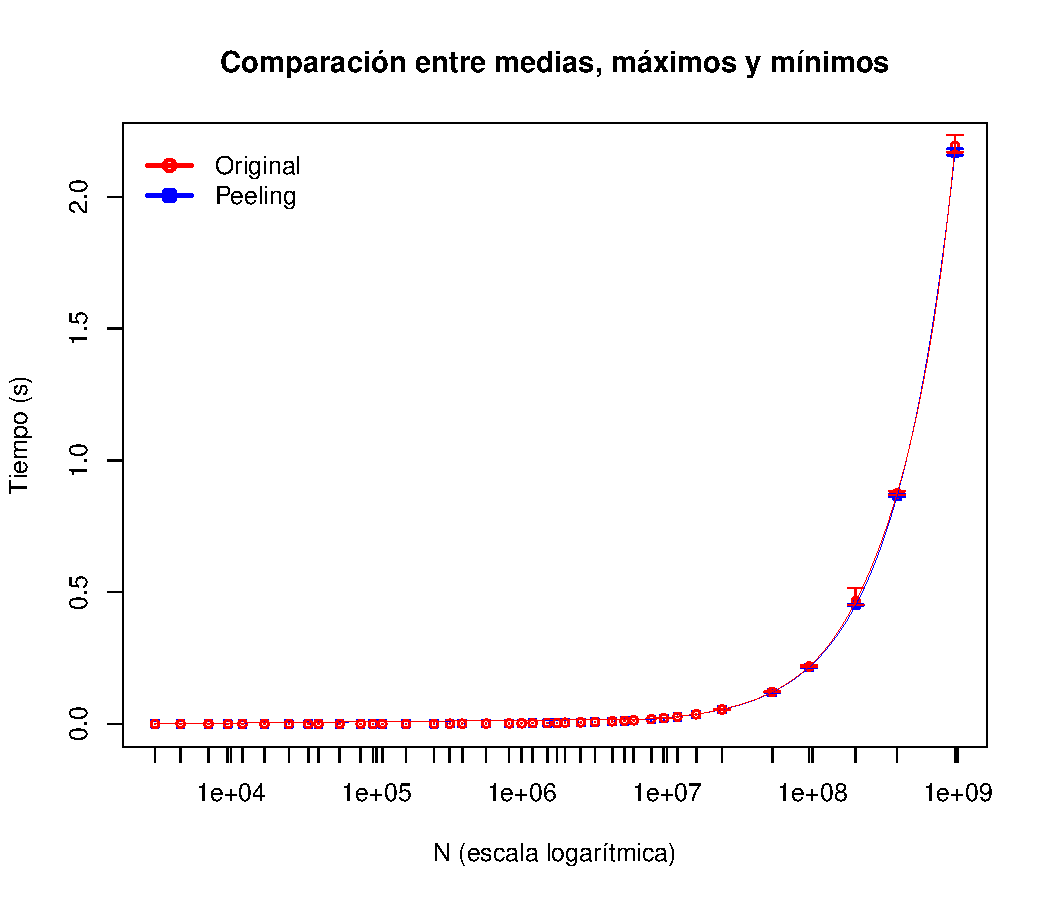
\includegraphics[width=.8\textwidth]{../graficas/DIA_tiempos.pdf}
		\caption{Comparativa global de los tiempos de ejecución.}
		\label{graf:tiempos}
	\end{figure}
	
	En la gráfica se aprecia que, aunque en justa y reducida medida, es claro que la versión con \textit{peeling} se ejecuta en un tiempo ligeramente menor para la mayoría de los distintos valores de \texttt{N}.
	
	\subsection{Aceleración}
	
	Una mejor manera de comparar las dos versiones del código es obtener la ganancia de una versión frente a la otra, es decir, la aceleración, que vendrá dada por:
	
	\begin{equation} \label{eq:speedup}
		ac = \dfrac{t_{\text{original}}}{t_{\text{peeling}}}.
	\end{equation}
	
	La Figura \ref{graf:speedup} implementa la expresión (\ref{eq:speedup}) tomando como referencia la media de tiempo de ejecución para cada \texttt{N}.
	
	Para cada tamaño de \texttt{N}, se consideran los tiempos de ejecución correspondientes a dos versiones distintas de un programa. Sea \( T_{\mathrm{OPT}}^{(N)} \) y \( T_{\mathrm{SIN}}^{(N)} \) los conjuntos de tiempos para cada versión. Se definen los cuantiles como \( Q_p(X) \), siendo \( Q_{0.25}(X) \) el cuantil inferior (primer cuartil) y \( Q_{0.75}(X) \) el cuantil superior (tercer cuartil) del conjunto \( X \). A partir de estos cuantiles, se estiman límites robustos para el \textit{speedup} como una franja entre dos cocientes: el inferior, que representa una ganancia conservadora, se calcula como:
	\begin{equation}\label{q1}
		\text{Speedup}_{\mathrm{min}} = \frac{Q_{0.25}(T_{\mathrm{SIN}}^{(N)})}{Q_{0.75}(T_{\mathrm{OPT}}^{(N)})},
	\end{equation}
	y el superior, que representa una ganancia potencial más optimista, como
	\begin{equation} \label{q2}
		\text{Speedup}_{\mathrm{max}} = \frac{Q_{0.75}(T_{\mathrm{SIN}}^{(N)})}{Q_{0.25}(T_{\mathrm{OPT}}^{(N)})}.
	\end{equation}
	
	Esta franja proporciona una estimación del rendimiento relativa entre ambas versiones, mitigando la influencia de valores atípicos.
	Viendo la gráfica de la Figura \ref{graf:speedup} es ya claro que la versión que utiliza \textit{peeling} se ejecuta ligeramente más rápido que la introducida inicialmente.
	
	\begin{figure} [H] \centering
		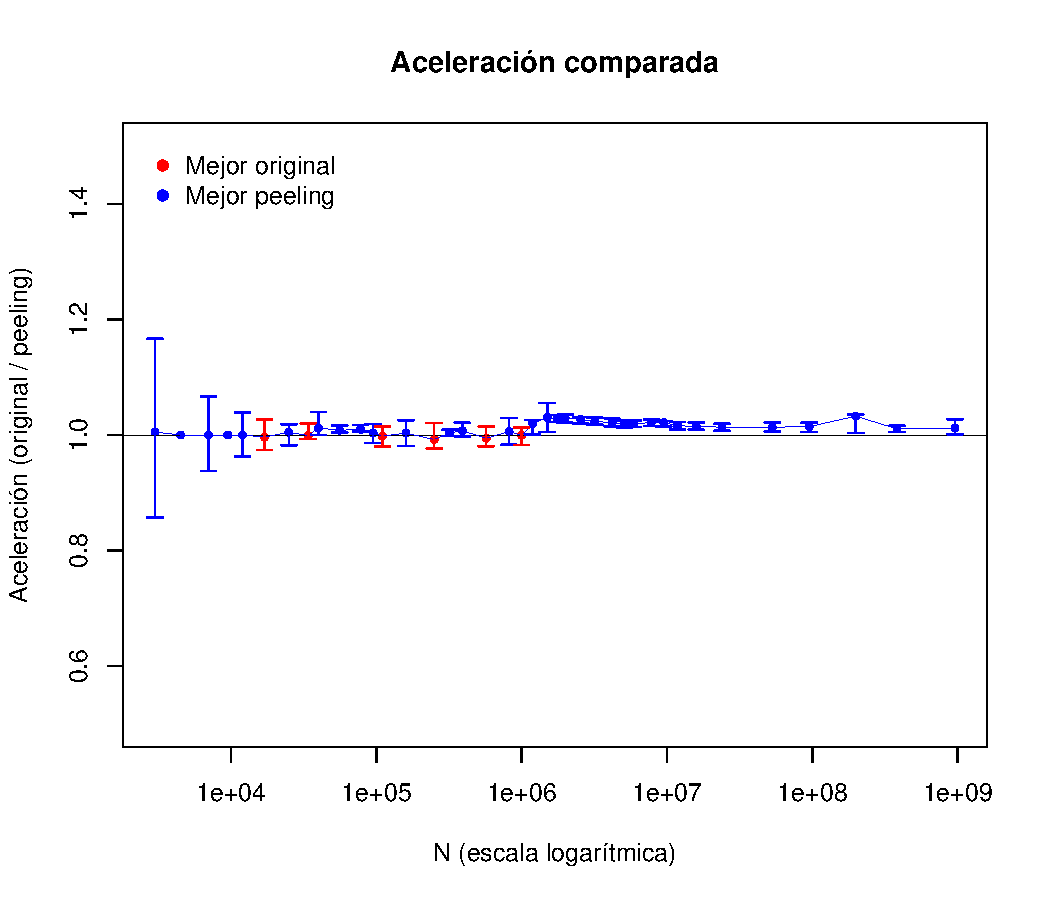
\includegraphics[width=.8\textwidth]{../graficas/DIA_speedup.pdf}
		\caption{Comparativa global de la aceleración media.}
		\label{graf:speedup}
	\end{figure}
	
	
	\section{Conclusiones}


\printbibliography
	
	
	

\end{document}